\documentclass{standalone}
\usepackage{tikz}

\begin{document}
	
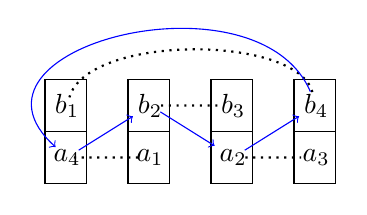
\begin{tikzpicture}[x=0.8pt,y=0.75pt,yscale=-1.25,xscale=1.25]
	\useasboundingbox  (-5pt,-15pt) rectangle (85pt,31pt);
	%cluster 1
	\def\x{30}
	\def\w{15}
	%Shape: Rectangle
	\draw   (0,0) -- (15,0) -- (15,40) -- (0,40) -- cycle ;
	%Straight Lines
	\draw   (0,20) -- (15,20) ;
	% Text Node
	\draw (8,10) node (b1)  {$b_{1}$} ;
	% Text Node
	\draw (8,30) node (a4)   {$a_{4}$};
	
	%cluster 2
	\draw   (\x,0) -- (\w+\x,0) -- (\w+\x,40) -- (\x,40) -- cycle ;
	\draw   (\x,20) -- (\w+\x,20) ;
	% Text Node
	\draw (\x+8,10) node (b2)   {$b_{2}$};
	% Text Node
	\draw (\x+8,30) node (a1)   {$a_{1}$};
	
	\draw[thick,dotted, shorten <= -6pt, shorten >= -6pt] (a4)  -- (a1);
	\draw [->,blue, shorten <= -5pt, shorten >= -2pt] (a4) -- (b2);
	
	%cluster 3
	\draw   (2*\x,0) -- (\w+2*\x,0) -- (\w+2*\x,40) -- (2*\x,40) -- cycle ;
	\draw    (2*\x,20) -- (\w+2*\x,20) ;
	% Text Node
	\draw (2*\x+8,10) node (b3)   {$b_{3}$};
	% Text Node
	\draw (2*\x+8,30) node (a2)   {$a_{2}$};
	\draw[thick,dotted, shorten <= -4pt, shorten >= -3pt] (b2)  -- (b3);
	\draw [->,blue, shorten <= -5pt, shorten >= -2pt] (b2) -- (a2);
	
	%cluster 4
	\draw   (3*\x,0) -- (\w+3*\x,0) -- (\w+3*\x,40) -- (3*\x,40) -- cycle ;
	\draw    (3*\x,20) -- (\w+3*\x,20) ;
	% Text Node
	\draw (3*\x+8,10) node (b4)   {$b_{4}$};
	% Text Node
	\draw (3*\x+8,30) node (a3)   {$a_{3}$};
	\draw[thick,dotted, shorten <= -4pt, shorten >= -3pt] (a2)  -- (a3);
	\draw [->,blue, shorten <= -5pt, shorten >= -2pt] (a2) -- (b4);
	
	\draw[thick, dotted,  shorten <= -3pt, shorten >= -5pt]  (b4) to[out=-100,in=-80] (b1);
	% arrow
	\draw[->, blue,shorten <= -3pt, shorten >= -4pt]  (b4) 
	to [out=-108,in=-130, distance=17mm]  (a4);
	\end{tikzpicture}
	
\end{document}